\documentclass{standalone}

%----------------------------------------------------------------------------------------------%
%                                 Packages and basic declarations
%----------------------------------------------------------------------------------------------%

\usepackage[utf8]{inputenc}
\usepackage{pgfplots}
\usepackage{tikz}


%----------------------------------------------------------------------------------------------%
%----------------------------------------------------------------------------------------------%
%                                            DOCUMENT STARTS
%----------------------------------------------------------------------------------------------%
%----------------------------------------------------------------------------------------------%

\begin{document}


%Tikz picture starts%

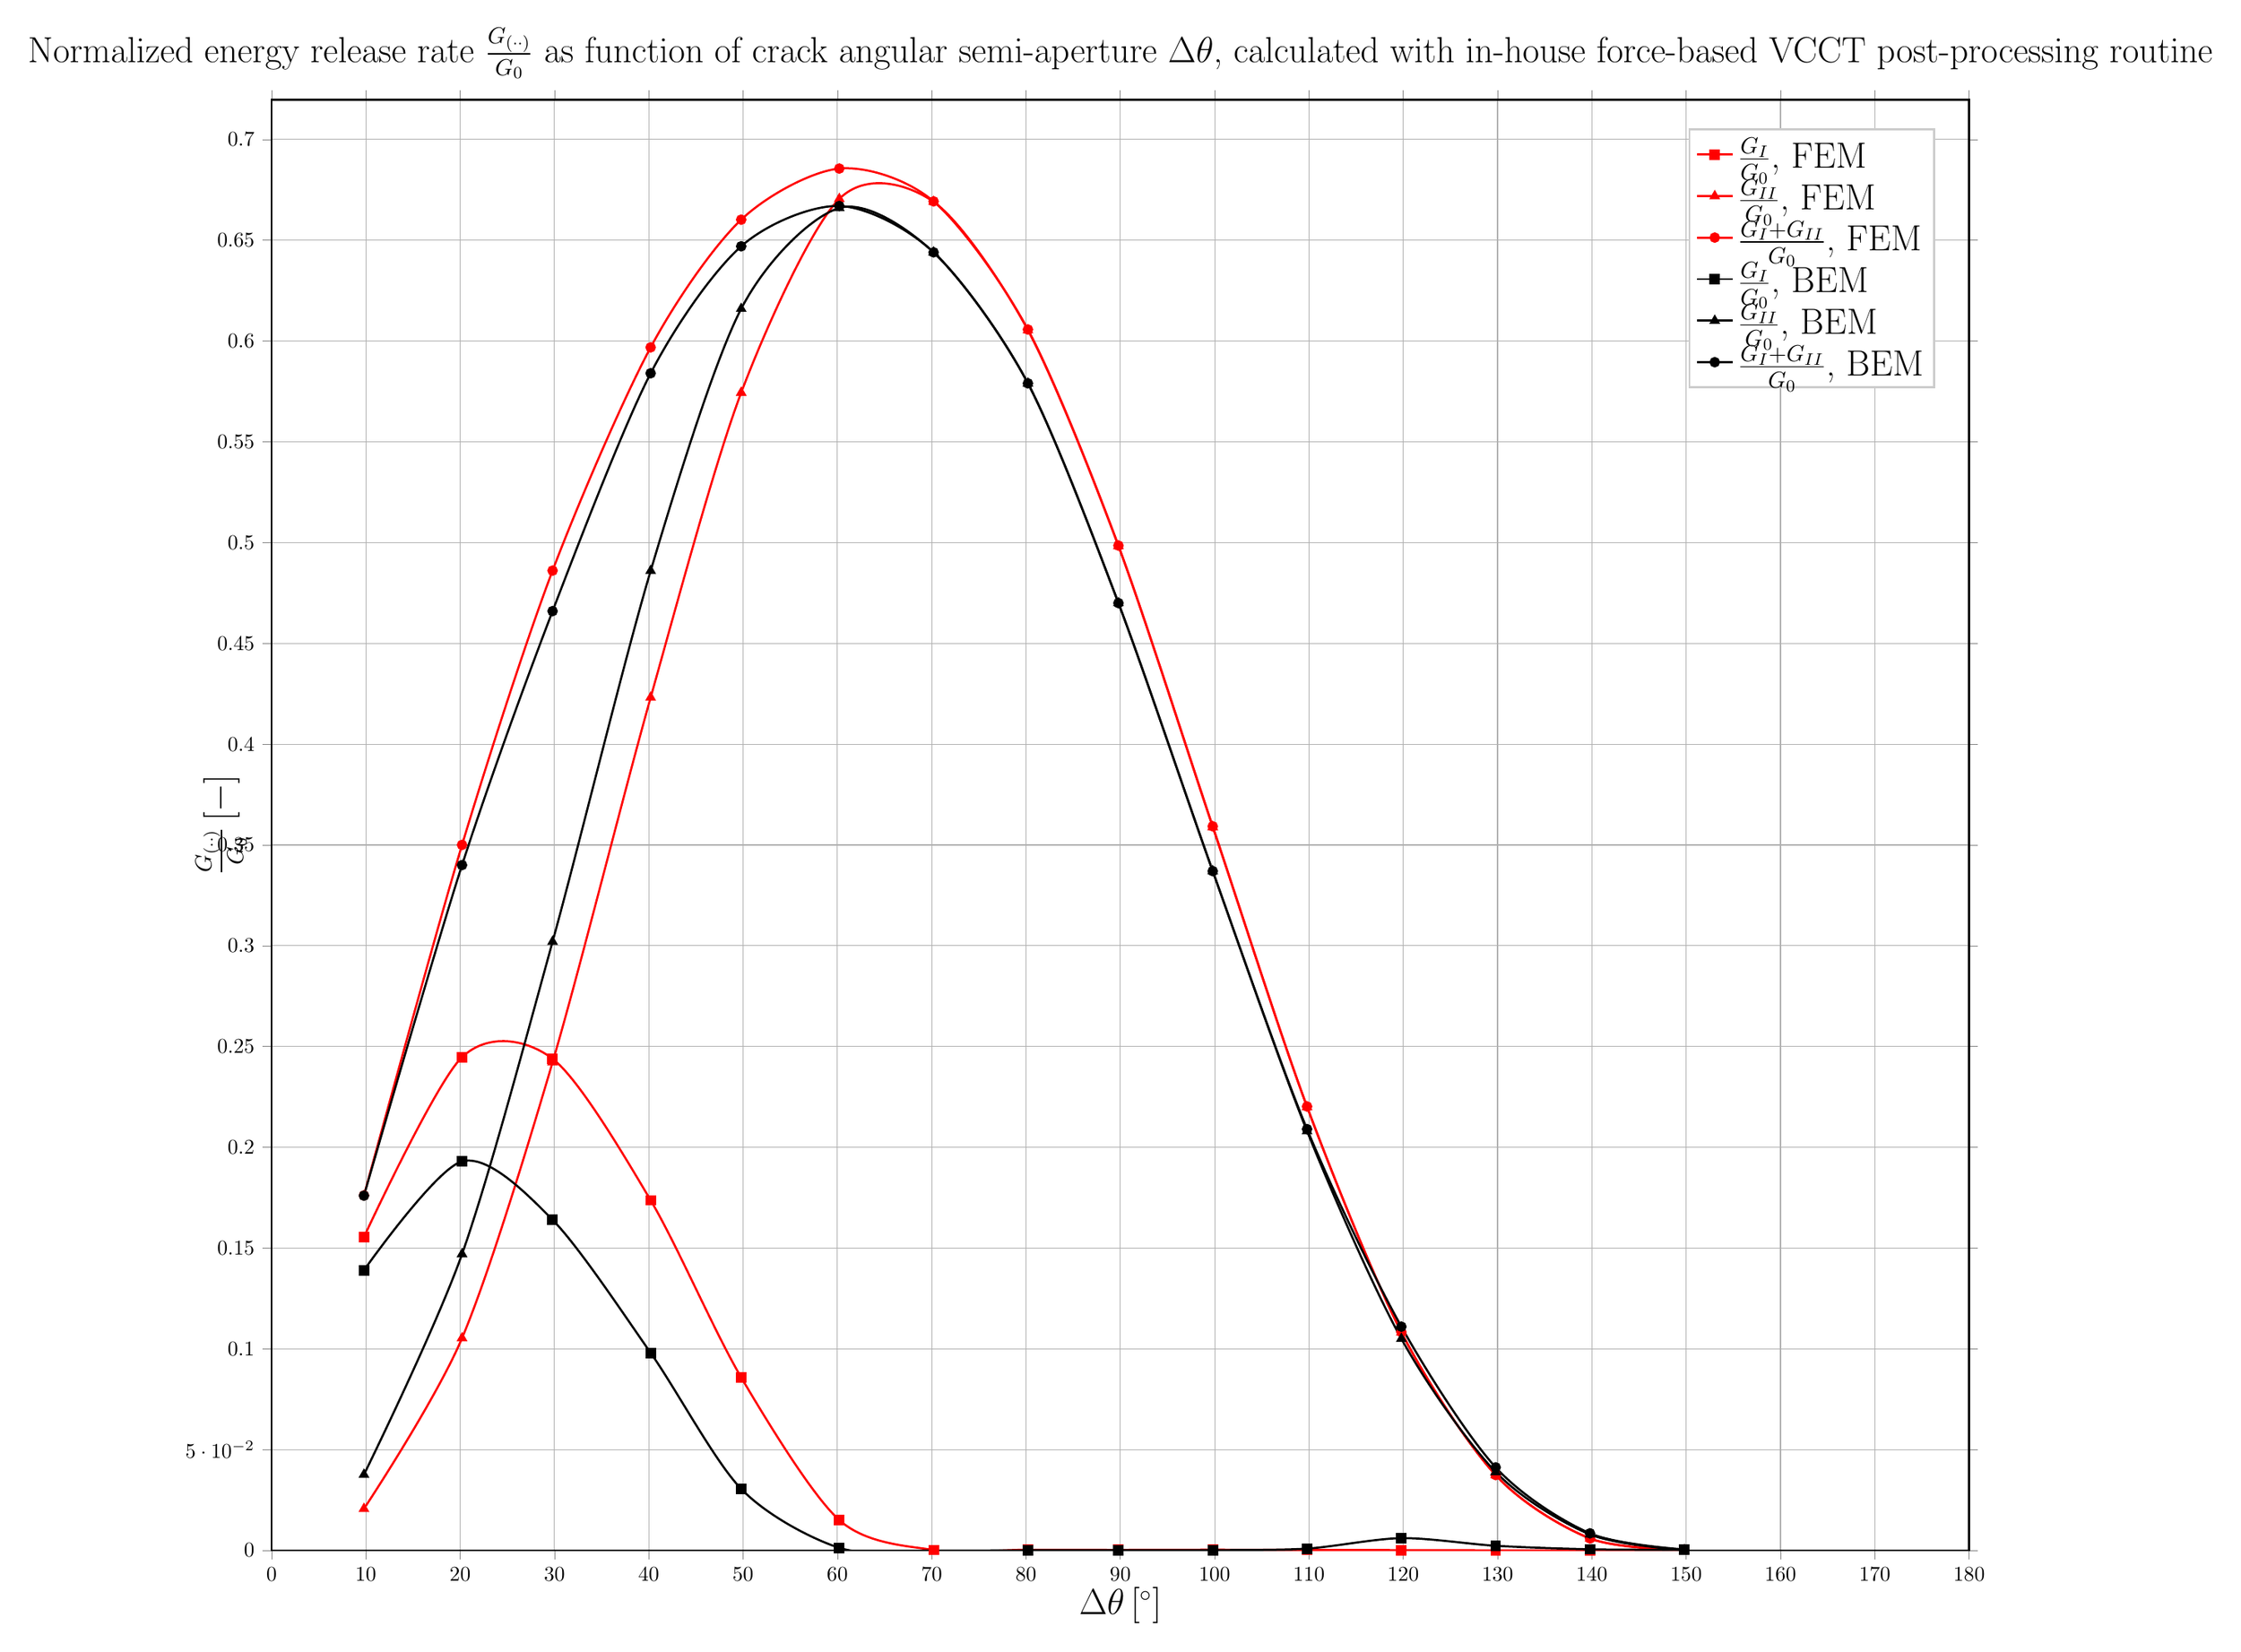
\begin{tikzpicture}

%Tikz axis starts%

\begin{axis}[width=30cm,
title={Normalized energy release rate $\frac{G_{\left(\cdot\cdot\right)}}{G_{0}}$ as function of crack angular semi-aperture  $\Delta\theta$, calculated with in-house force-based VCCT post-processing routine},
title style={font=\fontsize{16}{8}\selectfont},
xlabel style={at={(axis description cs:0.5,-0.02)},anchor=north,font=\fontsize{16}{8}\selectfont},
ylabel style={at={(axis description cs:-0.01,.5)},anchor=south,font=\fontsize{16}{8}\selectfont},
xlabel={$\Delta\theta\left[^{\circ}\right]$},ylabel={$\frac{G_{\left(\cdot\cdot\right)}}{G_{0}}\left[-\right]$},
xmin=0.0,
xmax=180.0,
ymin=0.0,
ymax=0.719842996686,
tick align=outside,
tick label style={font=\normalsize},
xtick={0.0,10.0,20.0,30.0,40.0,50.0,60.0,70.0,80.0,90.0,100.0,110.0,120.0,130.0,140.0,150.0,160.0,170.0,180.0},
xmajorgrids,
x grid style={lightgray!92.026143790849673!black},
ymajorgrids,
y grid style={lightgray!92.026143790849673!black},
line width=0.35mm,
legend style={draw=white!80.0!black,font=\fontsize{16}{12}\selectfont},
legend entries={{$\frac{G_{I}}{G_{0}}$, FEM},{$\frac{G_{II}}{G_{0}}$, FEM},{$\frac{G_{I}+G_{II}}{G_{0}}$, FEM},{$\frac{G_{I}}{G_{0}}$, BEM},{$\frac{G_{II}}{G_{0}}$, BEM},{$\frac{G_{I}+G_{II}}{G_{0}}$, BEM}},
legend cell align={left}
]

\addplot[red,smooth,mark=square*]
table{
9.8000083551 0.155460567628
20.2001564043 0.244697884439
29.7996713865 0.243913201752
40.1999526243 0.173693613831
49.8000464651 0.0858091094669
60.2003242878 0.0150431123073
70.1998714969 0.000211482065235
80.1999924418 0.000340765725736
89.799994075 0.000244897579994
99.8000057369 0.000349457750699
109.800126682 0.000233875602494
119.799673891 0.000144422884631
129.800136345 4.30288588979e-05
139.800052385 8.50729058977e-06
149.799859141 0.000344858180106
};

\addplot[red,smooth,mark=triangle*]
table{
9.8000083551 0.0206462384904
20.2001564043 0.105315569247
29.7996713865 0.242184394779
40.1999526243 0.423160114091
49.8000464651 0.574399309096
60.2003242878 0.670521646442
70.1998714969 0.669067394174
80.1999924418 0.605370090459
89.799994075 0.498267456802
99.8000057369 0.35887388231
109.800126682 0.219994429541
119.799673891 0.10819561778
129.800136345 0.0373345913184
139.800052385 0.00592173524266
149.799859141 5.62558429736e-05
};

\addplot[red,smooth,mark=*]
table{
9.8000083551 0.176106806118
20.2001564043 0.350013453685
29.7996713865 0.486097596531
40.1999526243 0.596853727922
49.8000464651 0.660208418563
60.2003242878 0.685564758749
70.1998714969 0.669278876239
80.1999924418 0.605710856185
89.799994075 0.498512354382
99.8000057369 0.35922334006
109.800126682 0.220228305143
119.799673891 0.108340040665
129.800136345 0.0373776201773
139.800052385 0.00593024253325
149.799859141 0.000401114023079
};

\addplot[black,smooth,mark=square*]
table{
9.8000083551 0.139
20.2001564043 0.193
29.7996713865 0.164
40.1999526243 0.098
49.8000464651 0.0305
60.2003242878 0.00127
70.1998714969 -4.79e-05
80.1999924418 6.85e-05
89.799994075 0.000112
99.8000057369 0.000112
109.800126682 0.000895
119.799673891 0.00607
129.800136345 0.00229
139.800052385 0.000552
149.799859141 0.000306
};

\addplot[black,smooth,mark=triangle*]
table{
9.8000083551 0.0376
20.2001564043 0.147
29.7996713865 0.302
40.1999526243 0.486
49.8000464651 0.616
60.2003242878 0.666
70.1998714969 0.644
80.1999924418 0.579
89.799994075 0.47
99.8000057369 0.337
109.800126682 0.208
119.799673891 0.105
129.800136345 0.0389
139.800052385 0.00792
149.799859141 0.000165
};

\addplot[black,smooth,mark=*]
table{
9.8000083551 0.176
20.2001564043 0.34
29.7996713865 0.466
40.1999526243 0.584
49.8000464651 0.647
60.2003242878 0.667
70.1998714969 0.644
80.1999924418 0.579
89.799994075 0.47
99.8000057369 0.337
109.800126682 0.209
119.799673891 0.111
129.800136345 0.0412
139.800052385 0.00847
149.799859141 0.000471
};

\end{axis}
%Tikz axis ends%


\end{tikzpicture}
%Tikz picture ends%


\end{document}

%----------------------------------------------------------------------------------------------%
%----------------------------------------------------------------------------------------------%
%                                            DOCUMENT ENDS
%----------------------------------------------------------------------------------------------%
%----------------------------------------------------------------------------------------------%

